% ------------------------------------------
% habitat count  & fish count 
% ------------------------------------------

\subsection{Habitat characteristics and preferences}

To answer/investigate the question if different species or genera of weakly electric fish prefer different (micro-) habitats, weakly electric fish were recorded in a network of river channels in the LLanos of the Orinoco basin, Meta, Colombia. For each recording the micro-habitat's characteristics were categorised. In total, within 13 larger habitats, 139 micro-habitat's characteristics, such as the presence or absence of stones, sand, mud, roots and plants, were denoted.\\
Within most (84~\%) of the examined micro-habitats  stones could be found frequently on the ground (fig.~\ref{fig:habitat_count}). In many micro-habitats  (35~\%) the stream bed was additionally or solely covered with sand. Roots could often (44~\%) been found on the shoreline, on the ground or as locked driftwood. Both, mud (6~\%) and plants (12~\%), were clearly more infrequent than other examined characteristics.\\
For each micro-habitat the species or genus of the recorded fish was determined. Over all 327 fish were recorded. \textit{Apteronotus} was by far the most frequent weakly electric fish. Approximately 250 of the recorded animals (76~\%) were identified as \textit{Apteronotus macrostomus}  (fig.~\ref{fig:fish_count_eod}~A). The EOD frequency of these animals ranged from approximately 560~to 1000~Hz and was slightly bimodal distributed (fig.~\ref{fig:fish_count_eod}~B). About 50 fish (15~\%) were identified as \textit{Eigenmannia virescens}. Their EODf mainly varied from 290~to 600~Hz. The less frequent fish with 20~(6~\%) recorded individuals were pulsefish. The EODf of this genus was less than 100~Hz.

\begin{figure}[H]
    \centering
    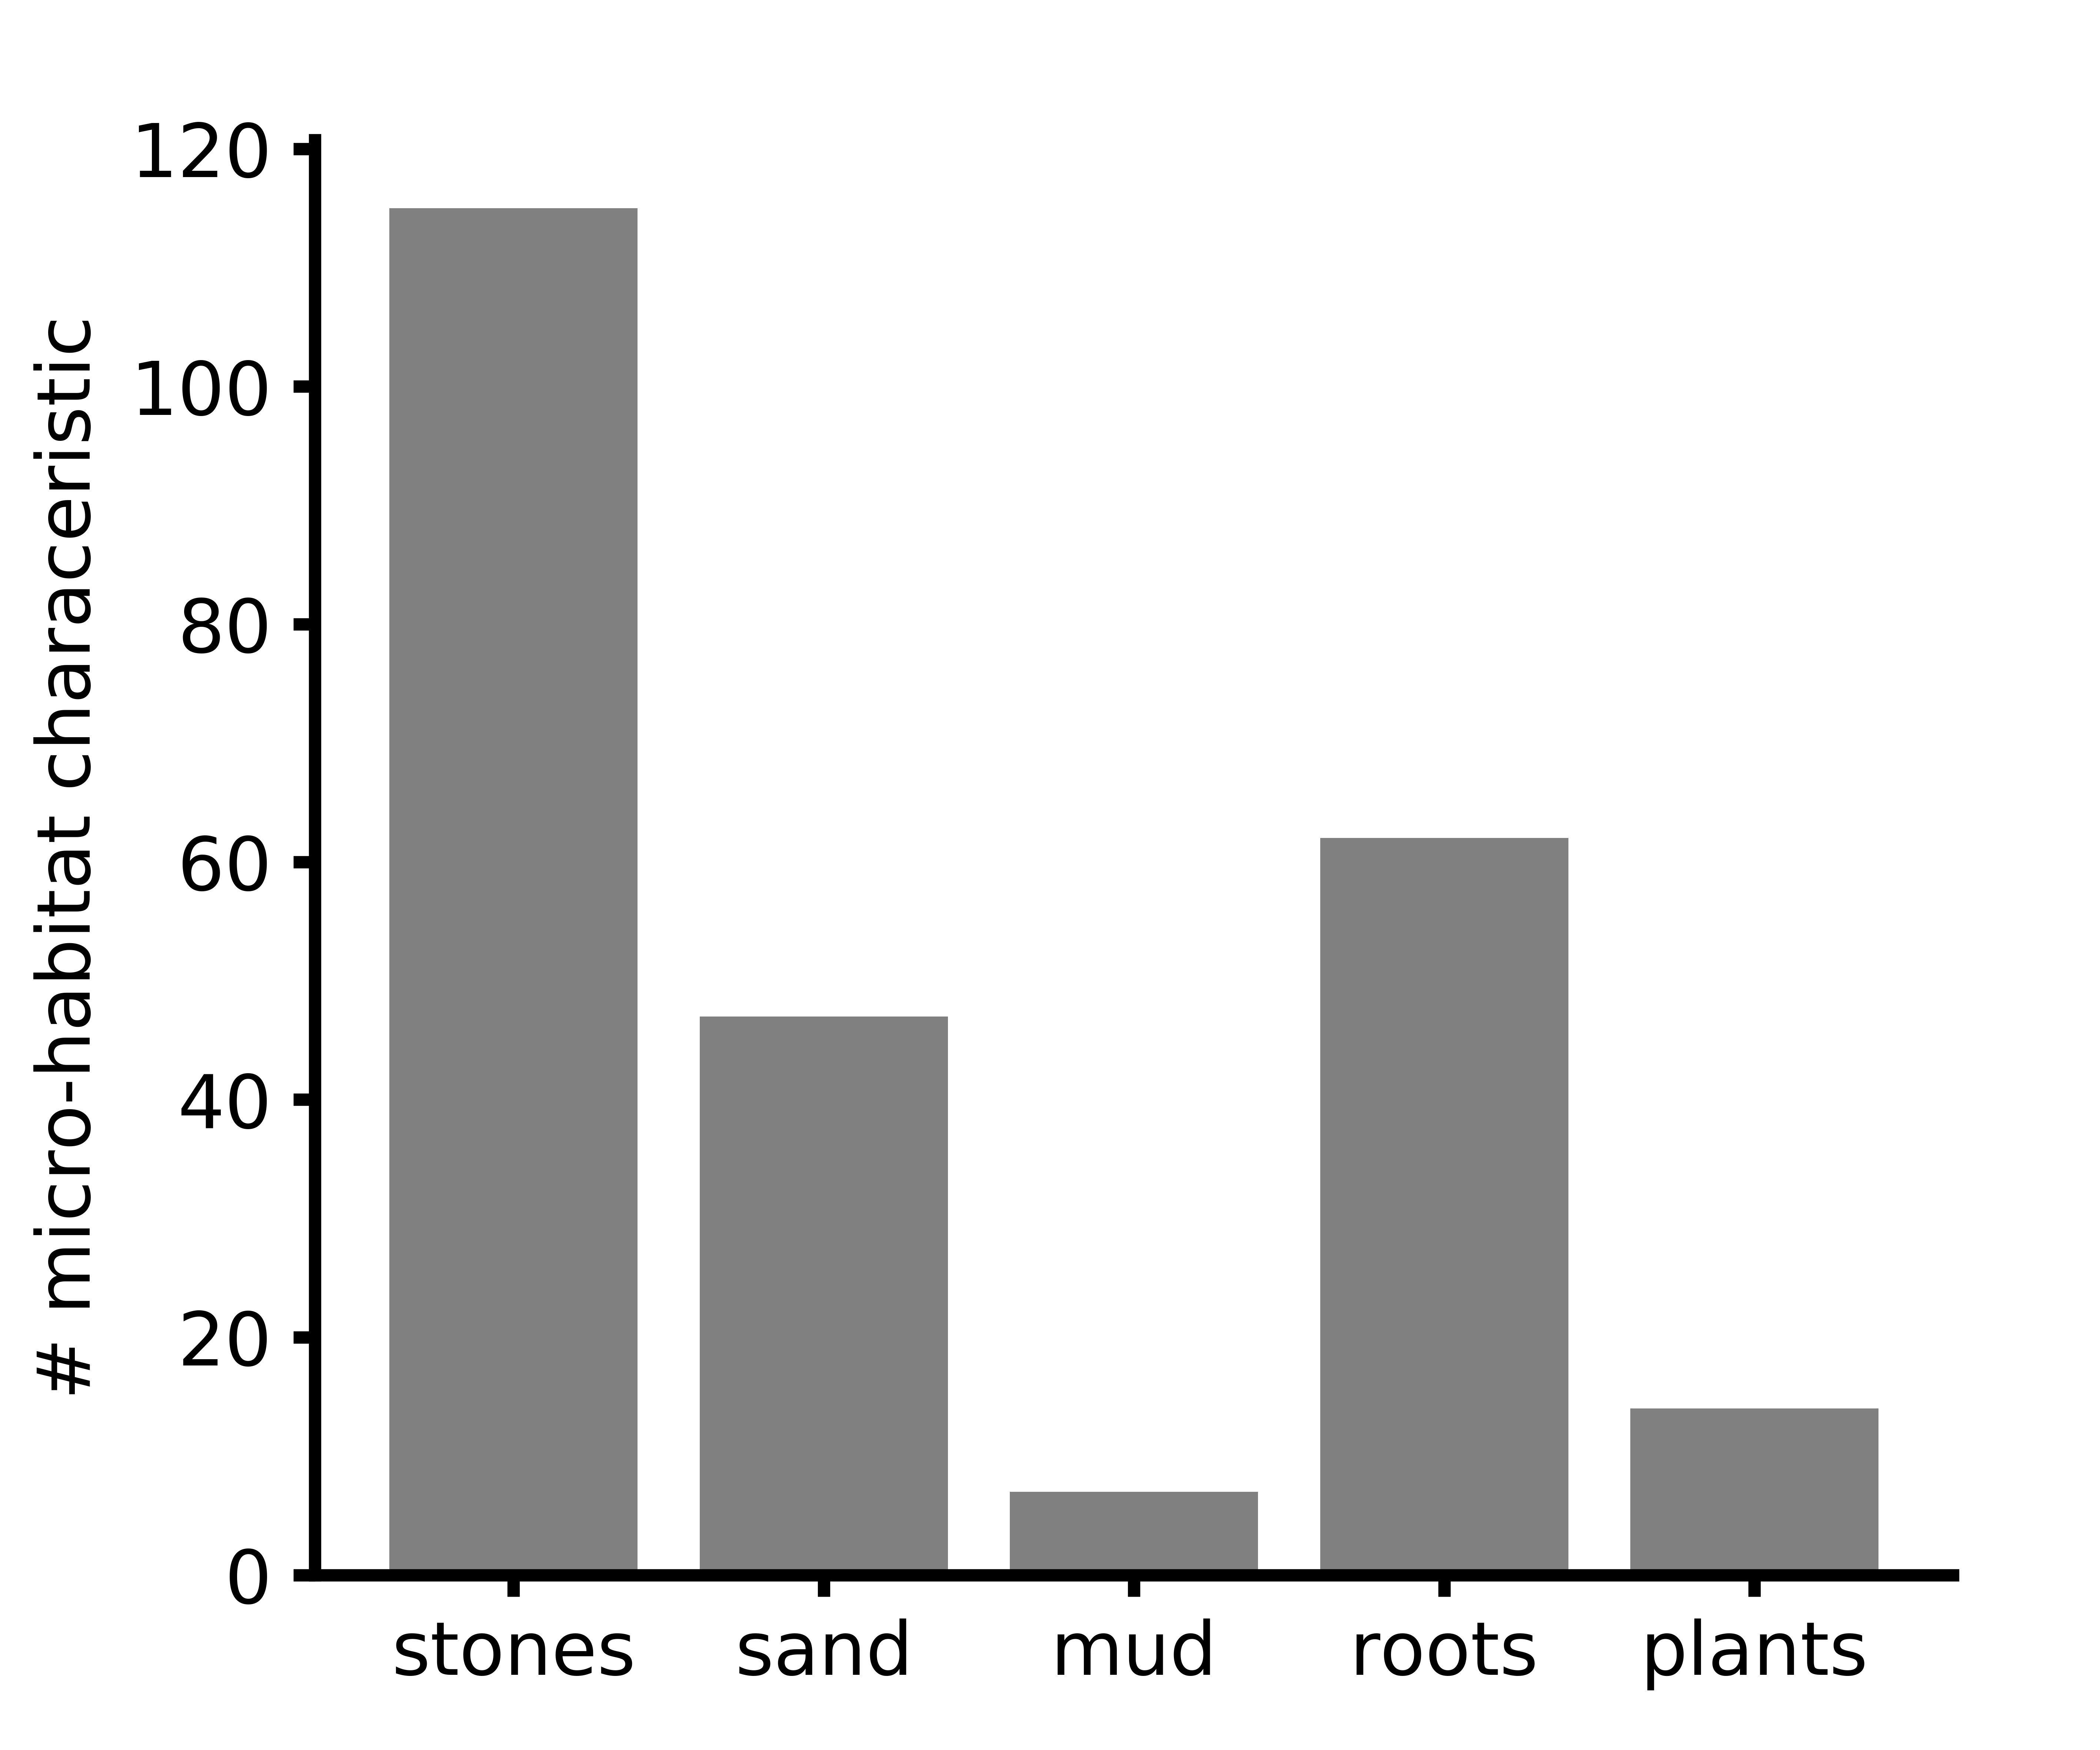
\includegraphics[width=0.65\textwidth]{pictures/Results/JULE_habitat_ccharacteristics.png}
    \caption{\textbf{Habitat characteristics.} Total count of micro-habitats in which stones, sand, mud, roots or different kinds of plants were found. A single micro-habitat could consist of multiple of these categories. Over-all, 139 micro-habitats were characterised.}
    \label{fig:habitat_count}
\end{figure}

\begin{figure}[H]
    \centering
    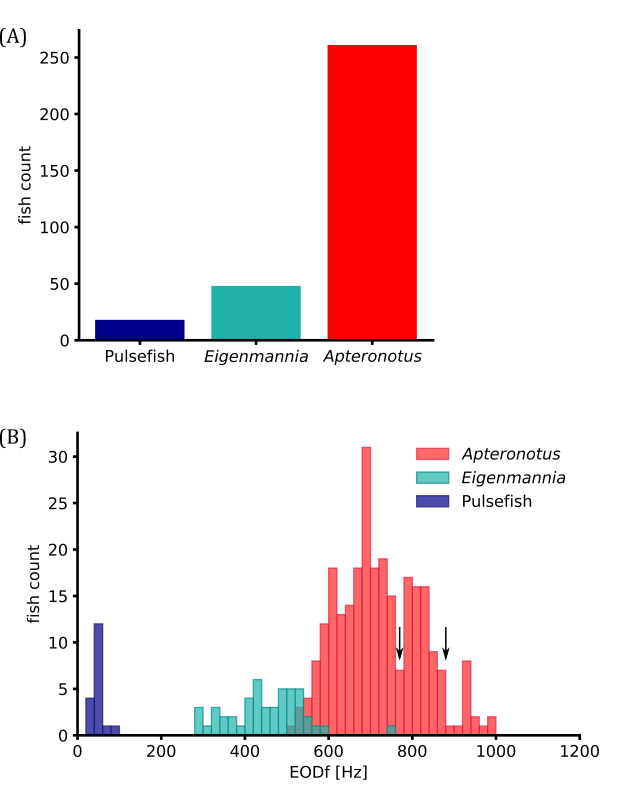
\includegraphics[width=0.9\textwidth]{pictures/Results/fish_count_EOD.png}
    \caption{\textbf{Proportion of fish species and EOD distribution.} \textbf{A:}~Shown is the number of animals we found within the 139 investigated micro-habitats for each species (\textit{Apteronotus macrostomus} and \textit{Eigenmannia virescens}) or genus (unknown pulsefish). \textbf{B:}~Distribution of the EOD frequencies (EODf) for each species or genus. In case of \textit{Apteronotus}, the first arrow (762~Hz) indicates the border between female and male individuals. The second arrow (880~Hz) indicates the border between males with lower dominance and highly dominant males.}
    \label{fig:fish_count_eod}
\end{figure}

% ---------------------------------------------
% species and habitats
% ---------------------------------------------

Regarding the average fish count dependent on the micro-habitat's characteristics, some preferences of the different species or genera can be seen, especially regarding \textit{Apteronotus} (fig.~\ref{fig:habitat_count_species}). On average, in each micro-habitat containing stones, two Apteronoti were found. Close to roots on average only one \textit{Apteronotus} was found. In micro-habitats with sand, mud and plants, this species was less frequent.
Also \textit{Eigenmannia} showed a slight preference for one of the habitat characteristics.
Most \textit{Eigenmannia}s were found in habitats with roots. On average the probability of finding an \textit{Eigenmannia} within a micro-habitat with roots was 75~\%. The probability of finding an individual of this species within a stony, sandy or muddy habitat reached from 25~to 50~\%. Not a single animal was found in a micro-habitat containing plants.
In contrast, most of the pulsefish, with a probability of 70~\%, were found in habitats with plants. The probability of finding a pulse-type fish within a micro-habitat containing sand, mud or roots ranged between 25~and 50~\%. Pulsefish were the less frequent in stony habitats.

\begin{figure}[H]
    \centering
    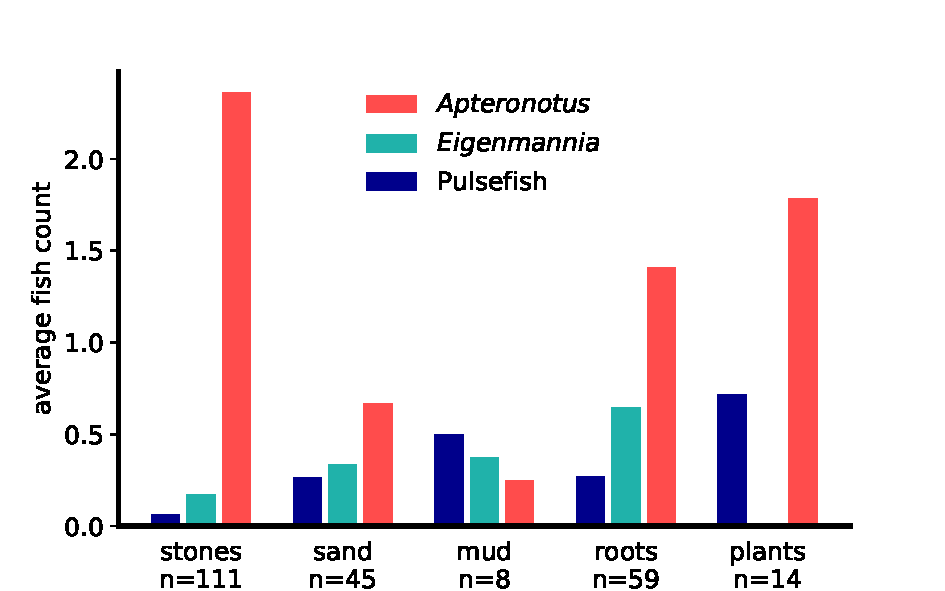
\includegraphics[width = \textwidth]{pictures/Results/average_occuranec_in_habitats.pdf}
    \caption{\textbf{Occurrance of species in the different micro habitats}\\
    Shown is the average fish count of Pulsefish (blue), \textit{Eigenmannia virescens} (cyan) and \textit{Apteronotus macrostomus} (red) in an micro-habitat with certain characteristic. Micro-habitats could contain many different characteristic elements. Hence a single micro-habitat and the corresponding, recorded animals can occur more than once in the figure. Average count corresponds with the probability to occure in a certain habitat.}
    \label{fig:habitat_count_species}
\end{figure}

\begin{figure}[H]
    \centering
    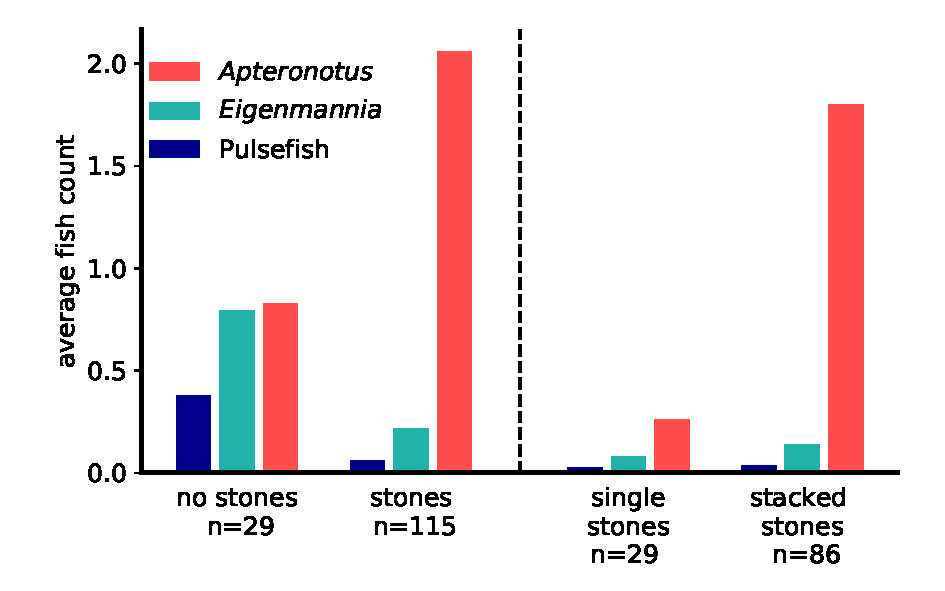
\includegraphics[width = \textwidth]{pictures/Results/more_stones_pls.pdf}
    \caption{\textbf{Preference of species to stony habitats.} Average count of fish for Pulsefish (blue), \textit{Eigenmannia virescens} (cyan) and \textit{Apteronotus macrostomus} (red) found in micro-habitats with and without stones (left) and average count in the subdivision of stony habitats in single stones and stacked stones (right). }
    \label{fig:habitat_count_stones}
\end{figure}

Next we solely looked at the occurrence of the fishes in stony habitats and habitats without stones (fig.~\ref{fig:habitat_count_stones}). Both, \textit{Eigenmannia} and pulsefish showed no preference for habitats with stones. However, \textit{Eigenmannia virescens} was more likely to be found in habitats with stacked stones than in habitats with separate stones. A clear preference could be found for \textit{Apterontus macrostomus}. This species was most likely found in micro-habitats containing stacked stones.

\begin{figure}[H]
    \centering
    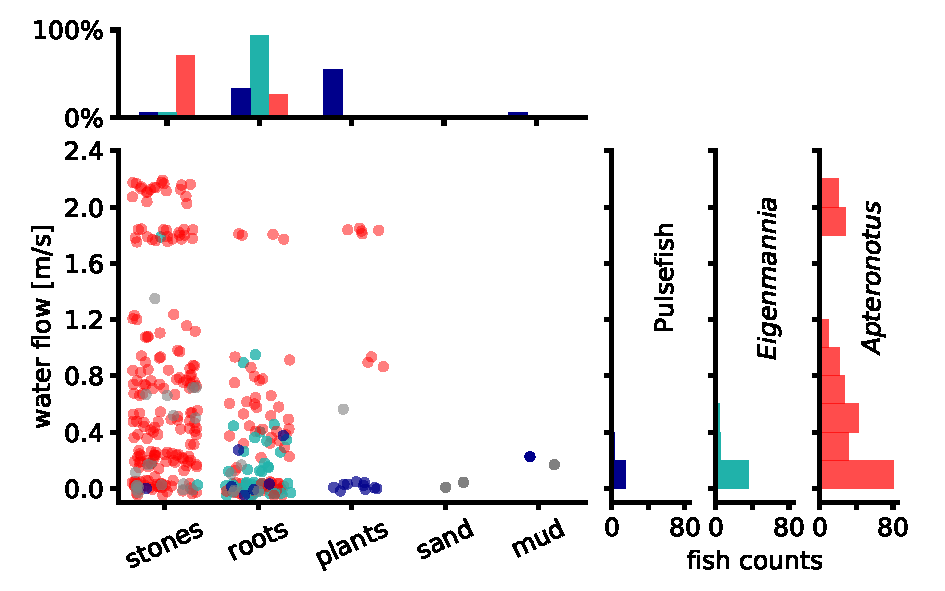
\includegraphics{pictures/Results/flow_habitat_protocol.pdf}
    \caption{\textbf{Distribution of the different fish species over the water flow in different micro-habitats.} On the top, for the species \textit{Apteronotus} (red) and \textit{Eigenmannia} (cyan) and the genus of pulsefish (blue) the distribution in the different habitats is shown. The bottom left figure shows the distribution of the fishes in the different habitats over the water flow. The areas with no recorded fish (grey) are shown as well. The habitats are ranked according to the observations in the field. Habitats with roots were ranked above stones, while plants are ranked above roots. If there were neither roots nor plant nor stones, mud was preferred over sand (plants~$>$~roots~$>$~stones~$>$~mud~$>$~sand). The three histograms on the bottom right, show the distribution of the species over the water flow.}
    \label{fig:habitat_vs_flow}
\end{figure}

In contrary to the previous results, in figure~\ref{fig:habitat_vs_flow} every fish is only represented once. Additionally, different micro-habitats are ranked based on the observation of the experimenter. The ranking considered that plants are preferred over roots, but if there are no roots and plants, stones were preferred over mud. If there were neither roots nor plant nor stones nor mud, sandy habitats were occupied (plants~$>$~roots~$>$~stones~$>$~mud~$>$~sand). Mud and sand were considered as less attractive habitats, because they offer less hiding spaces.\\

Besides the ground conditions, the water flow and the water depth was measured in each micro-habitat. Comparing the ground conditions and the water flow, a clear difference in preference between the species could be seen. Figure \ref{fig:habitat_vs_flow} shows that pulse fish could be found in micro-habitats with a slow water flow (water flow $<$ 0.37 m/s) (median: 0.0~m/s) and preferably in micro-habitats with plants, but also in habitats with sand and roots. \textit{Eigenmannia} also prefers a water flow of a median of 0~m/s and could mainly be found in habitats with roots. In contrast, \textit{Apteronotus} preferred a median water flow of 0.42 m/s. Especially in stony micro-habitats, it could be seen that \textit{Apteronotus} rested where the water flow raised up to 2.15~m/s. 
It couldn't be shown, that there was one specific micro-habitat were always fish could be found. But it could be shown that, if there was a sandy habitat, there were no fish.

\begin{figure}[H]
    \centering
    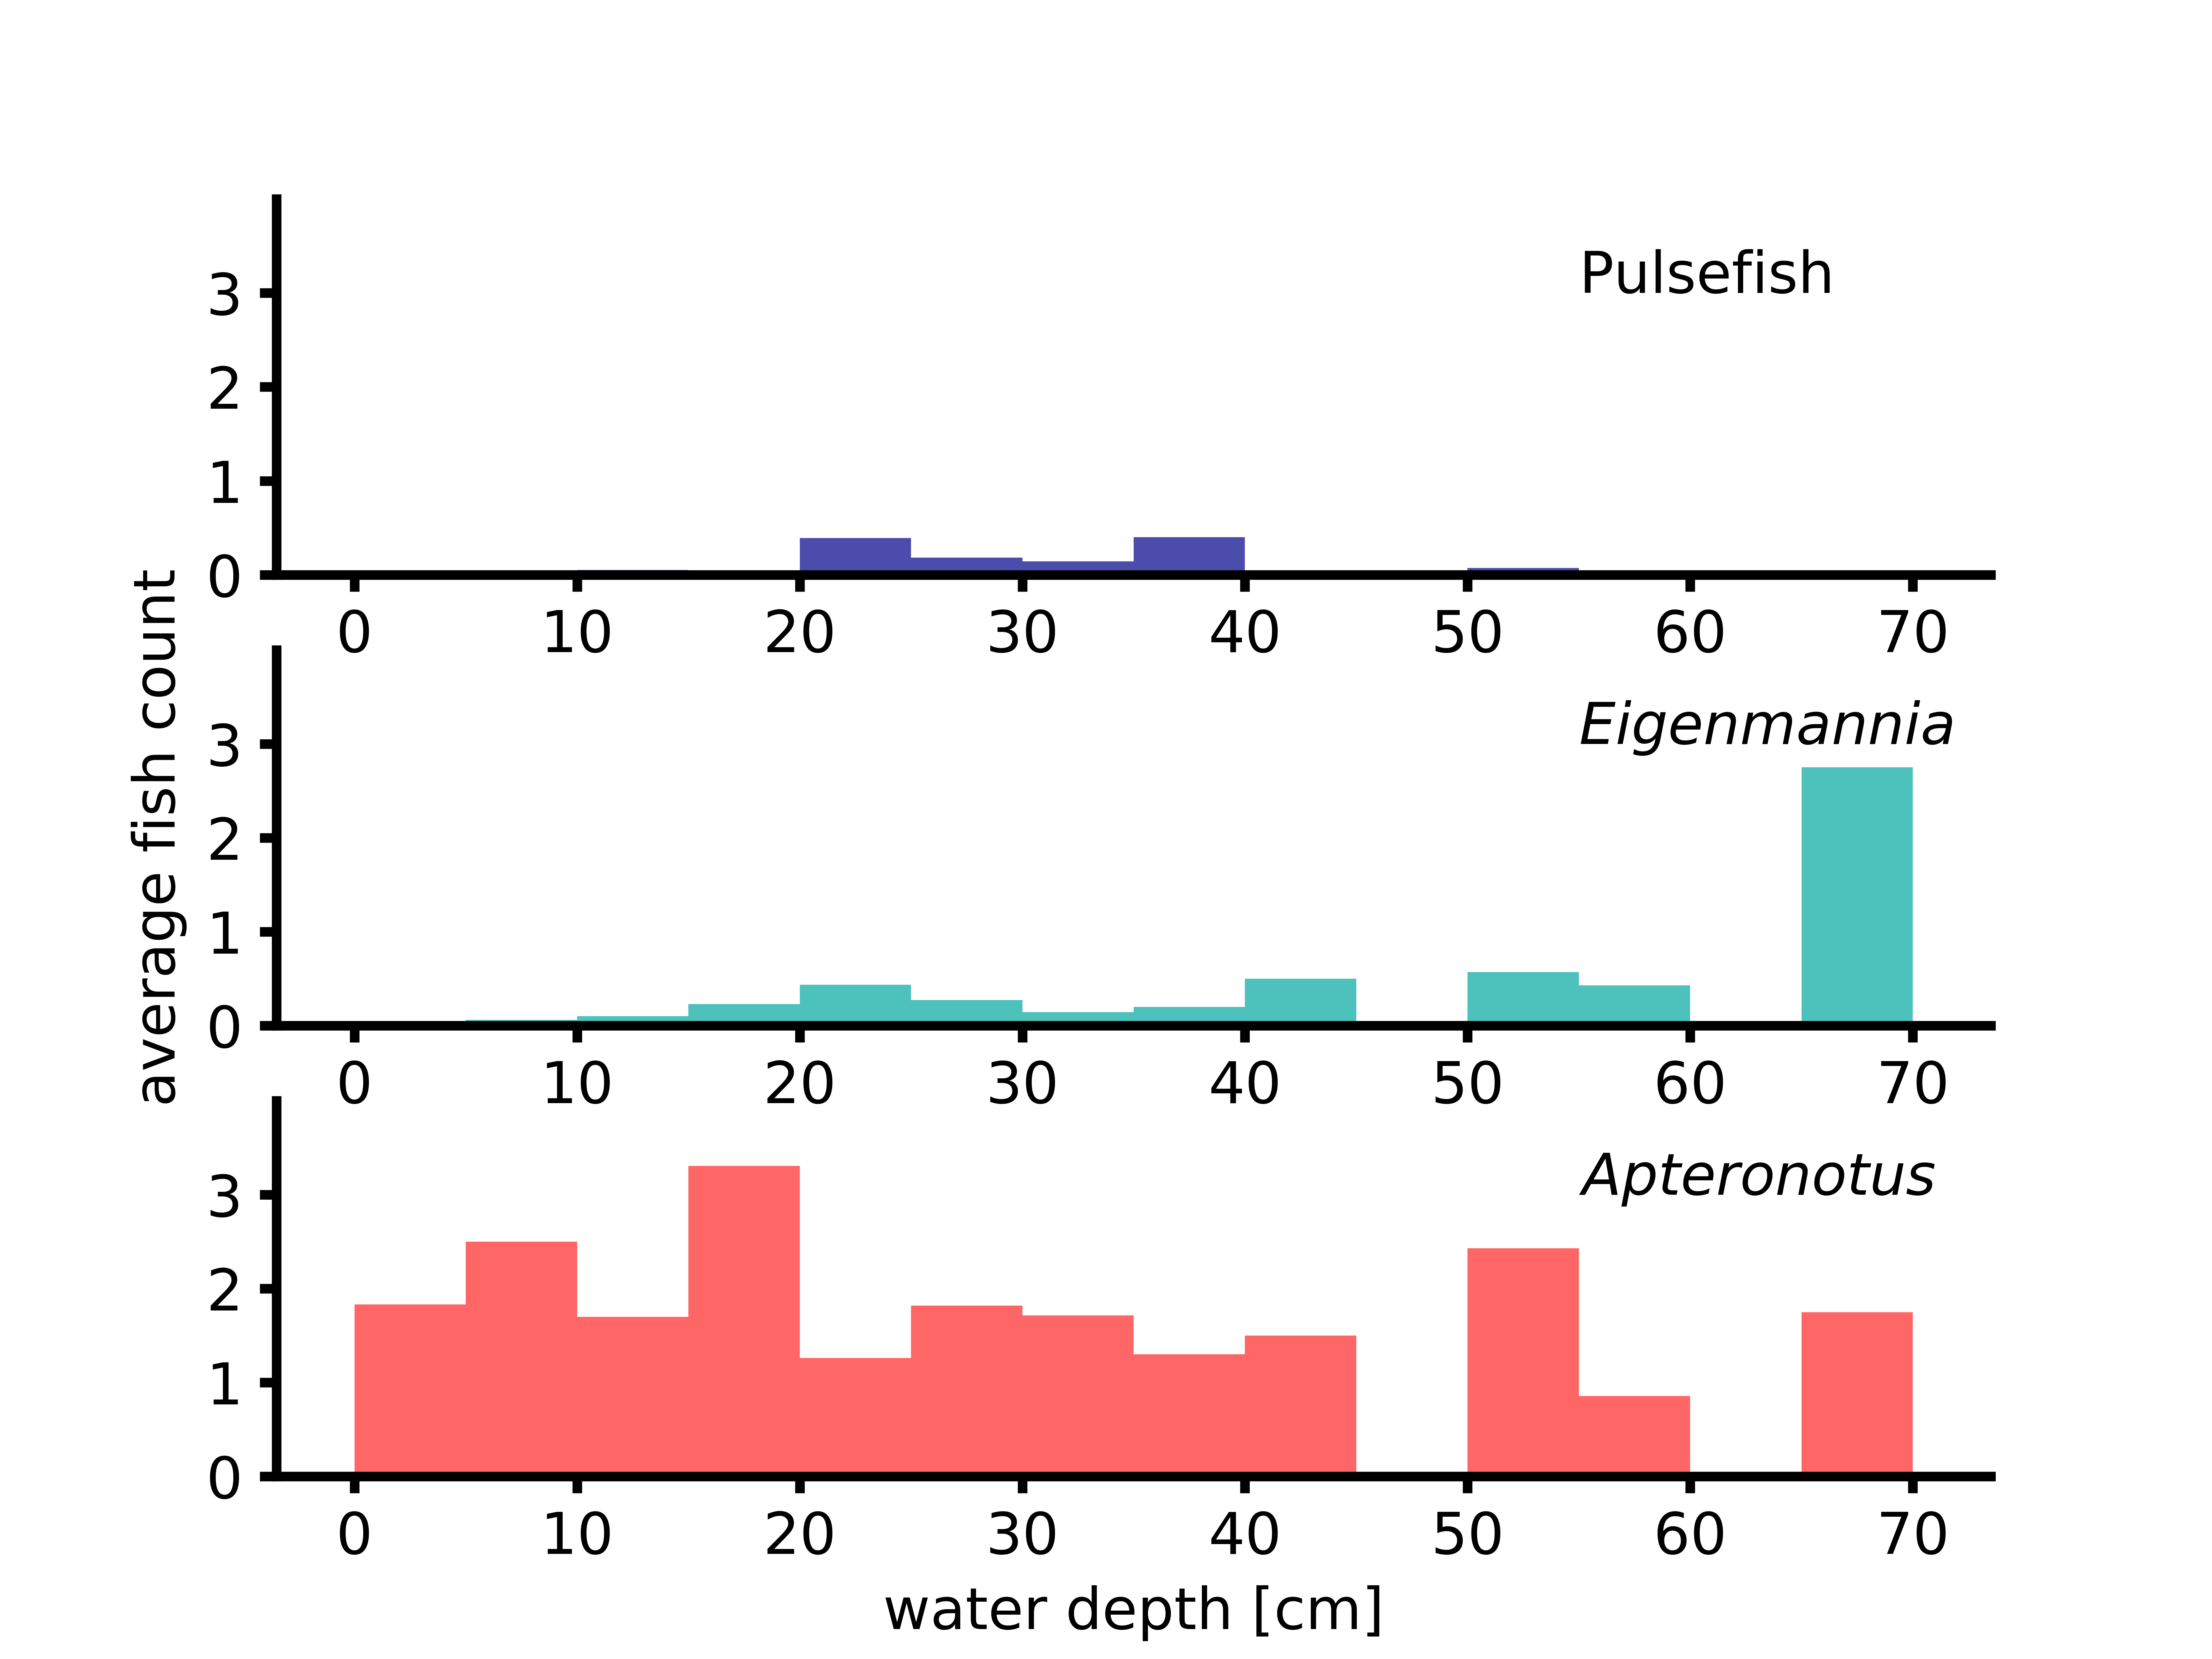
\includegraphics[width=0.9\textwidth]{pictures/Results/JULE_flow_depth2.png}
    \caption{\textbf{Occurrence of species dependent on water depth.} Shown is the average fish count for micro-habitats within a certain range of water depth for pulsefish (blue), \textit{Apteronotus macrostomus} (red) and \textit{Eigenmannia virescens (cyan)}.}
    \label{fig:habitat_vs_depth}
\end{figure}

In addition to the occurrence of the different species or genera dependent on the water flow, also their occurrence dependent on the water depth was investigated. Micro-habitats with a water depth of 45~to 50~cm and 60~to 65~cm were not found. Regarding \textit{Apteronotus} and pulsefish, no preference for a certain water depth can be seen (fig.~\ref{fig:habitat_vs_depth}). Pulsefish were found in habitats with a water depth between 10~and 55~cm. Apteronoti were found in micro-habitats with a water depth ranging from a few centimeters up to 70~cm. Also \textit{Eigenmannia} was found within a large range of water depth (5~to 70~cm). In contrast to the other species or genera, \textit{Eigenmannia virescens} seemed to appear more frequently in habitats with a water depth between 65~and 70~cm.


% ----------------------------------------------
% Apteronoti (male / female) 
% ----------------------------------------------

\subsection{Dominance and habitat preferences in \textit{Apteronotus}}

\begin{figure}[H]
    \centering
    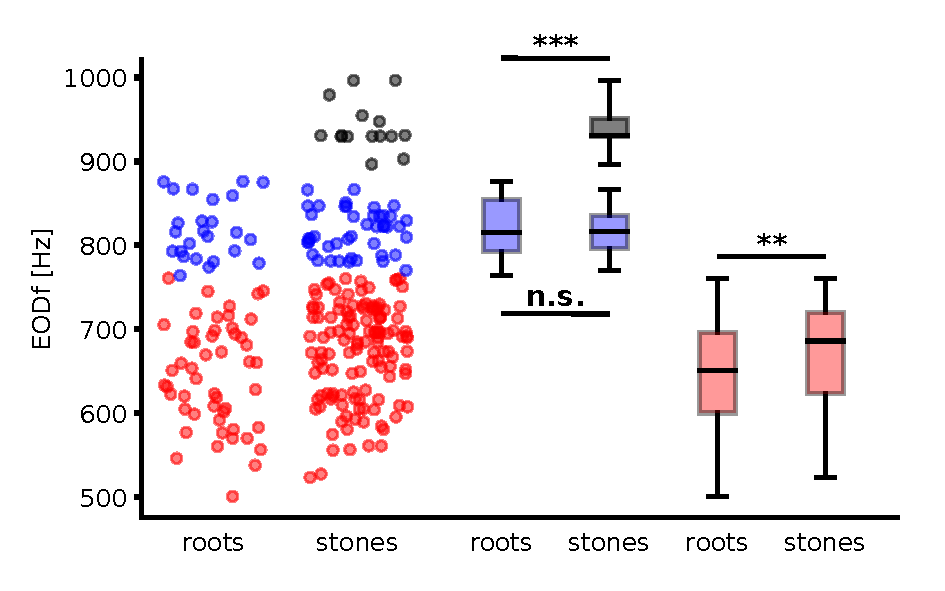
\includegraphics{pictures/Results/eod_habitat.pdf}
    \caption{\textbf{Distribution of the different EODfs of \textit{Apteronotus}, depending on the root and stone micro-habitats.} Distribution of male and female \textit{A. macrostomus} in root habitats and stone habitats. Based on the over-all EOD distribution in figure \ref{fig:fish_count_eod}, males had an EODf above 762 Hz. The males were also divided into high frequency males and low frequency males at a threshold of 880 Hz.}
    \label{fig:habitat_vs_eod}
\end{figure}

It could be shown that many \textit{Apterontus macrostomus} can be found in micro-habitats made of stones or roots. This leads to the question how males and females occupy the different micro-habitats. Females and males were found in both, stone and root micro-habitats (fig.~\ref{fig:habitat_vs_eod}). According to the EOD distribution in fig.~\ref{fig:fish_count_eod}B, the male \textit{A. macrostomus} can be divided into low frequency and high frequency (above 880~Hz) males. For those height frequency males it can be shown that, they could be found exclusively in stony habitats. Low frequency males do not prefer roots or stones (Man-Whitney-U-Test: U = ..., p = 0.003).
Females do prefer stony habitat over roots (Man-Whitney-U-Test: U = ..., p = ...). \textcolor{red}{DISCUSSION: Based on the common knowledge that males with a high EOD frequency are dominant, it can be assumed that stony habitats are the preferred hiding place during the day.}